% #############################################################################
% This is Chapter 5
% !TEX root = ../main.tex
% #############################################################################
% Change the Name of the Chapter i the following line
\fancychapter{Implementation and Evaluation}
% The following line allows to ref this chapter
\label{chap:evaluation}

This chapter gives an overview of the implementation of the compiler, which is covered on the first section, as well as the testing strategy, on the second section, and the performance evaluation strategy and results, on the third section.

The compiler has been fully implemented in Java, within the existing \ac{CLASS} and \ac{SAM} interpreters code base. The implementation follows the architecture described in \Cref{chap:architecture}, and includes all the optimizations described in \Cref{chap:optimizations}.

The implementation has been extensively tested through a bench of more than 180 incremental unit tests written in the \ac{CLASS} language, covering all language features. Additionally, multiple existing \ac{CLASS} programs used to test the original interpreters have also been incorporated into the test suite.

The performance of the generated code has been evaluated through a benchmark program and the results compared with different compiler configurations, the interpreted execution of the same program using both the \ac{CLASS} and \ac{SAM} interpreters, and an equivalent implementation in Haskell.

\section{Implementation}

The compiler is contained within a new \texttt{compiler} namespace within the existing \ac{CLASS} and \ac{SAM} interpreters Java code base. The main class of the compiler is \texttt{Compiler}, which orchestrates the different compilation phases. This compiler is invoked through a bash script, which also invokes \texttt{gcc} to generate the final executable from the generated C code.

The compiler starts by parsing flags and options from the command line. Each of the implemented optimizations is toggled by a flag, making it possible to easily benchmark the impact of each optimization. It is also possible to configure the target architecture (e.g., 32-bits or 64-bits), enable trace logs on generated programs, enable the printing of the \ac{IR} program at different stages, among other options.

The input \ac{CLASS} source code is parsed and type-checked using the original code, generating an annotated \ac{AST}. The \ac{AST} is visited by the \texttt{IRGenerator} visitor, producing an \ac{IR} program, as described in \Cref{section:IRGeneration}. Enabled optimizations are then applied, and finally, the optimized \ac{IR} program is translated to C code through the \texttt{CGenerator} visitor, as described in \Cref{section:IRtoC}.

The \ac{IR} is modeled as a set of classes representing the different instructions, expressions, and slots, following the model described in \Cref{section:IR}. Each instruction class provides methods to accept visitors, as well methods to easily transform the instructions during the optimization phases. While \texttt{IRExpression} objects occur as fields of \texttt{IRInstruction} objects, the latter are stored within \texttt{IRBlock} objects. An \texttt{IRProcess} object contains a description of the process header, and a set of labeled \texttt{IRBlock} objects, one of them being the entry block. Finally, an \texttt{IRProgram} object contains a set of \texttt{IRProcess} objects.

On the C generation phase, a number of helper classes are used to make both the compiler code more readable and maintainable, as well as to generate simpler C code. The \texttt{CSize} and \texttt{CAlignment} classes represent a size and alignment in bytes, respectively, and provide methods to perform arithmetic operations. The results of these operations are simplified as much as possible automatically, making the generated code easier to read. The memory layouts of various data structures are represented by classes such as \texttt{CProcessLayout}, which hold the offsets and alignments of each field, as well as the total size and alignment of the structure. Memory layouts are generated by visiting the slot trees generated during the \ac{IR} generation phase, which themselves were generated by visiting the \ac{AST} types.

\section{Testing the compiler}

The project repository includes a comprehensive suite of more than 180 unit tests written in the \ac{CLASS} language, which cover all features of the language, including edge cases relevant to the implemented optimizations. Each test is composed of a \ac{CLASS} source file, and optionally, a number of input and expected output files. Tests are categorized into folders based on the language feature they cover, such as exponentials, polymorphism, or process calls.

Multiple complex \ac{CLASS} programs, both existing ones and newly written (such as game of life and merge sort) were also integrated into the test suite, in addition to the smaller unit tests, in order to further validate the correctness of the generate code when many features are combined.

In order to easily find memory errors, a compiler flag \texttt{--profiling} can be enabled to compile the programs with allocation counters for each type of structure (e.g., processes, tasks, exponentials) and report any memory leaks when the program finishes execution. Additionally, the compilation script supports passing flags to \texttt{gcc} to enable the address and thread sanitizers, helping find and troubleshoot memory access errors and data races.

Tests are executed through a bash script \texttt{test\_compiler.sh}, which runs each test in the suite, with an optional filter to select specific tests. The script compiles each test using the available debugging flags. If successfully compiled, and if input files are provided, the generated executable is run for each input file and the output is compared with the expected output file (if provided). If there are no input files, the executable is simply run to check for runtime errors. The script reports the results of each test, including compilation errors, runtime errors, memory leaks, and output mismatches. Compiler flags can also be passed to the script to test different configurations. To speed up the testing process, tests are distributed across multiple jobs.

\section{Performance evaluation}

To measure the performance of the compiler, three benchmarking CLASS programs were developed along with equivalent Haskell implementations. Different compiler configurations were benchmarked, including the interpreted execution of the same program using both the \ac{CLASS} and \ac{SAM} interpreters, and the equivalent Haskell implementations, compiled with GHC \texttt{-O2}. All presented results are averaged over 10 runs, and were obtained on a machine with an Intel Core i9-12900K CPU and 32GB of RAM, running NixOS 25.05. The full benchmark results are presented in \Cref{chapter:appendixResults}.

\begin{figure}
    \centering
    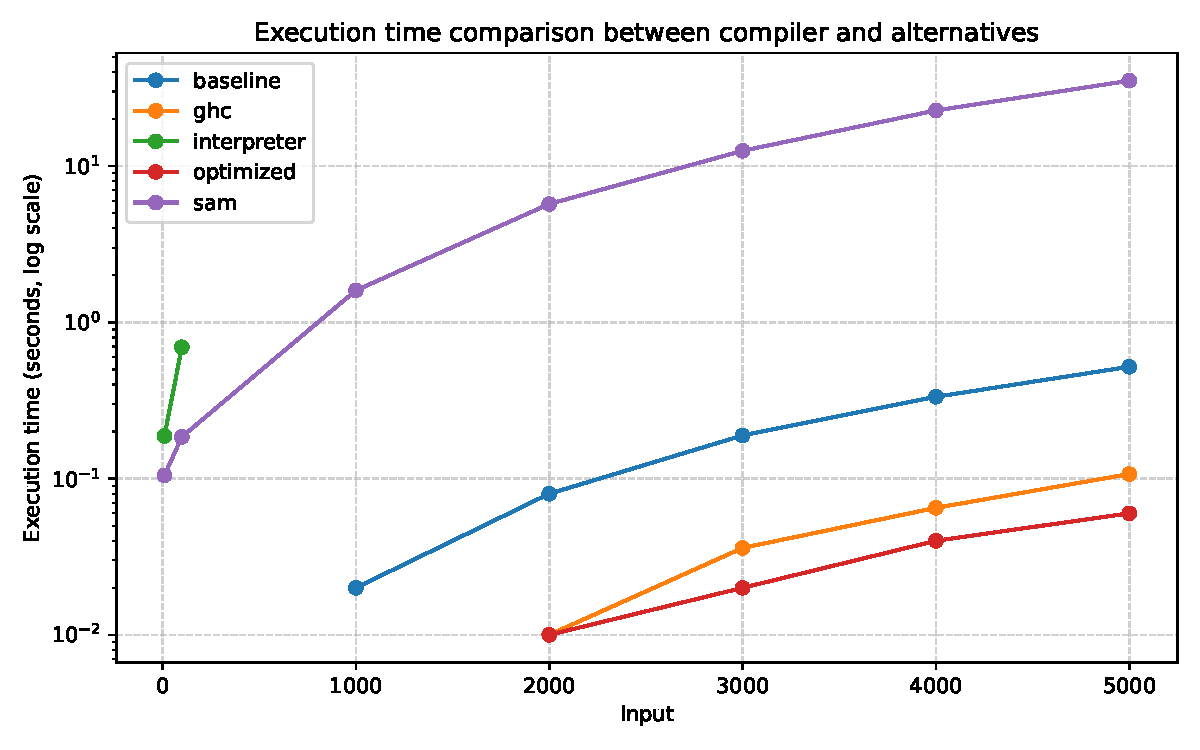
\includegraphics[width=0.49\textwidth]{./Images/execution_time_sieve_compiler_vs_alternatives.pdf}
    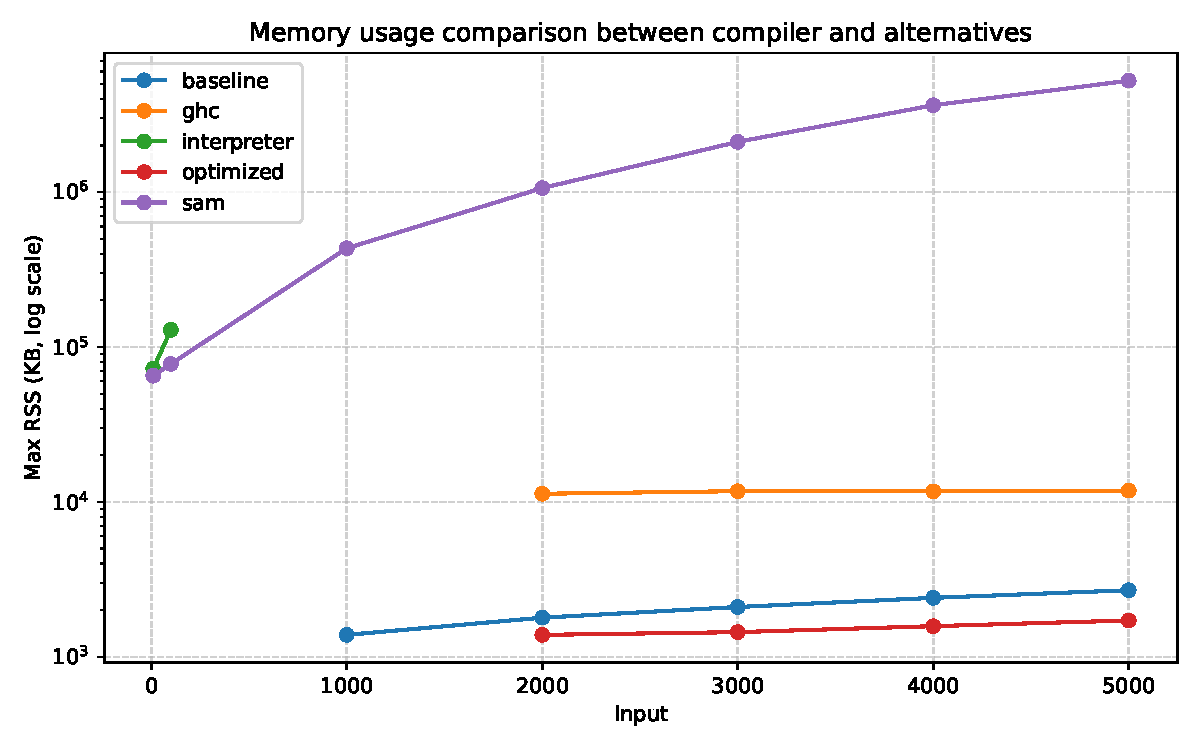
\includegraphics[width=0.49\textwidth]{./Images/memory_usage_sieve_compiler_vs_alternatives.pdf}
    \caption{Prime sieve benchmarks averaged over 10 runs, parametrized over prime count. Compares the original interpreter, the SAM, the baseline compiler, the compiler with all optimizations enabled, and GHC.}
    \label{fig:SieveBenchmarkCompilerVsAlternatives}
\end{figure}

The first benchmark program computes prime sieve numbers using the Turner's Sieve algorithm, generating a list of prime numbers up to a given count, taken as input. This benchmark was chosen because it is a simple yet computationally intensive program. On \Cref{fig:SieveBenchmarkCompilerVsAlternatives}, the execution time and the maximum \ac{RSS}, representing the peak memory usage, are compared between the original \ac{CLASS} interpreter, the \ac{SAM} interpreter, the unoptimized (baseline) compiler, the fully optimized compiler, and the equivalent Haskell implementation. The original interpreter cannot handle more than 150 primes due to operating system limits on the number of threads. The results show that the fully optimized compiler achieves a speed up of more than 100x compared to the \ac{SAM} interpreter, a speedup of more than 5x compared to the unoptimized compiler, and also that it outperforms the Haskell implementation, while using significantly less memory.

\begin{figure}[H]
    \centering
    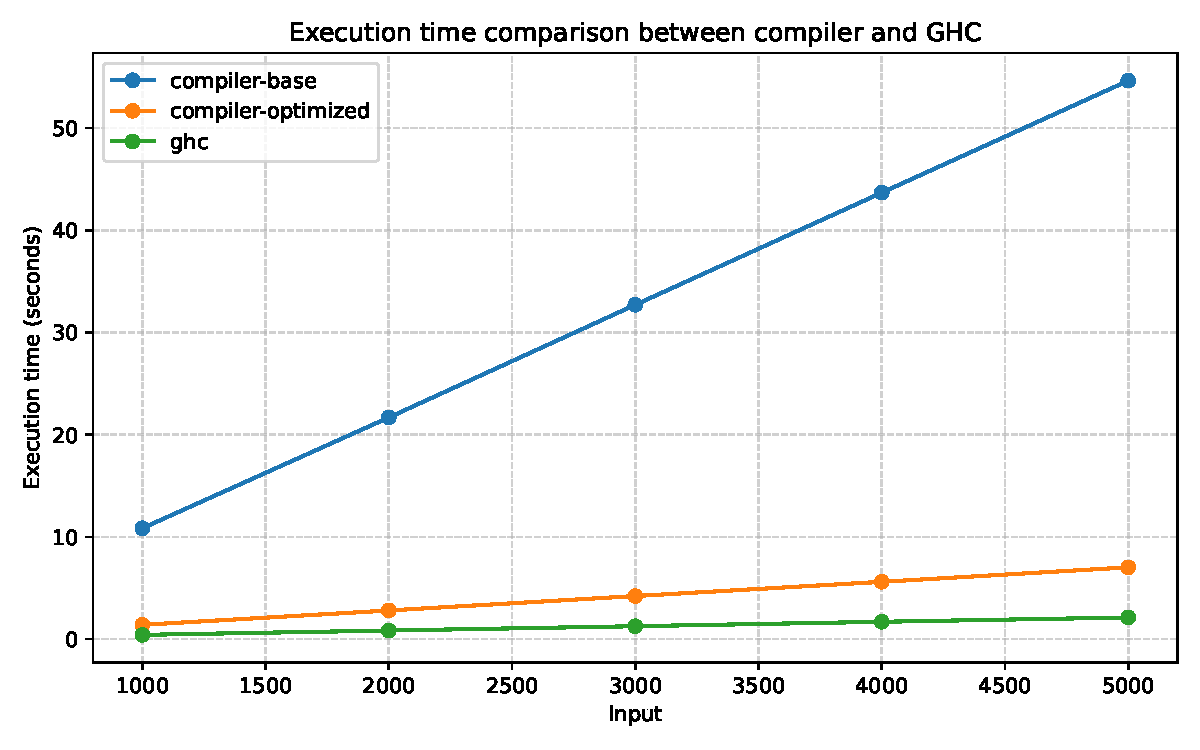
\includegraphics[width=0.49\textwidth]{./Images/execution_time_gol_compiler_vs_ghc.pdf}
    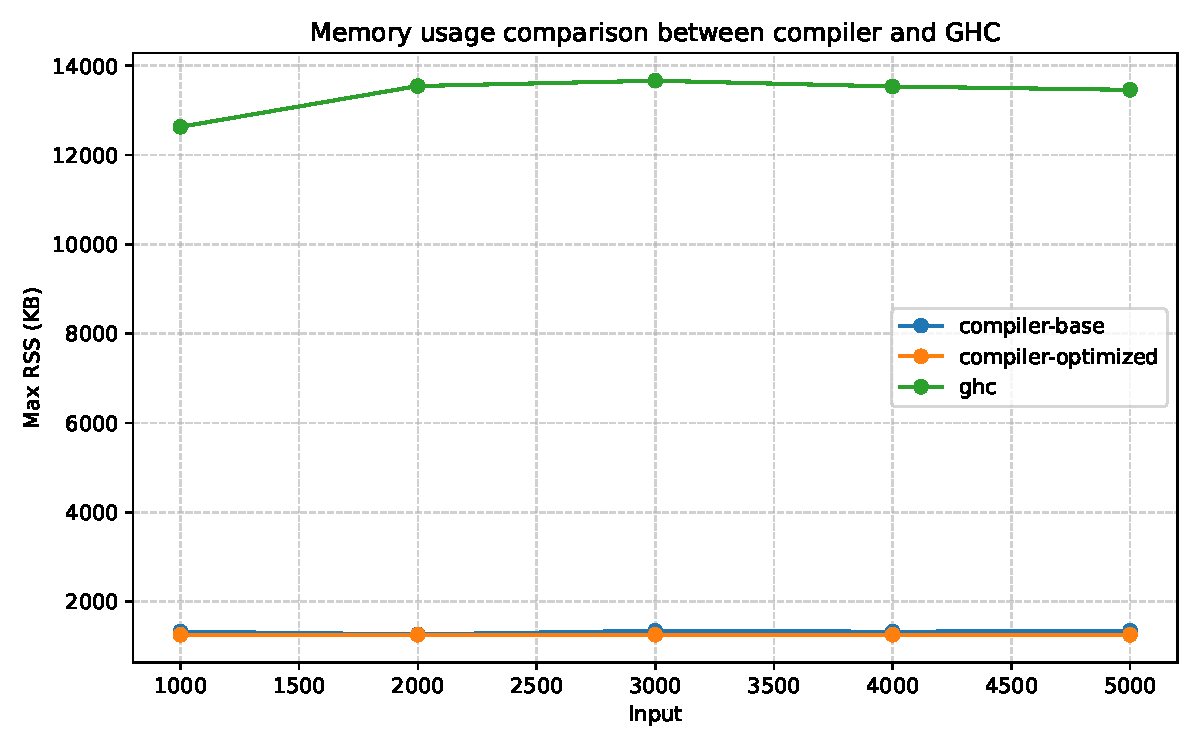
\includegraphics[width=0.49\textwidth]{./Images/memory_usage_gol_compiler_vs_ghc.pdf}
    \caption{Game of Life benchmarks averaged over 10 runs, parametrized over generation count. Compares the baseline compiler, the compiler with all optimizations enabled, and GHC. Both the original interpreter and the SAM were unable to run this benchmark.}
    \label{fig:GOLBenchmarkCompilerVsGHC}
\end{figure}

The second benchmark program implements a functional version of the Game of Life cellular automaton \cite{GameOfLife:1970}. All runs were given the same 17x17 initial configuration containing the \textit{Kok's galaxy}\cite{KoksGalaxy} pattern, and were parametrized by the number of generations to compute. In this benchmark, shown in \Cref{fig:GOLBenchmarkCompilerVsGHC}, the optimized compiler performs slower than the Haskell implementation, by a factor of approximately 2.5x. The memory usage of the generated program is, however, significantly lower than the Haskell implementation. We suspect that with further optimizations, such as allocating data in registers and reusing sessions and data sections, the Haskell implementation can be matched or even surpassed.

A third benchmark, covering the shared state features of \ac{CLASS}, implements a queue shared between a producer and a consumer. The producer pushes a number of items into the queue, while the consumer pops them concurrently. The Haskell implementation uses \texttt{MVar} to implement the shared state, as it bears a strong resemblance to the cells of \ac{CLASS}. The results, shown in \Cref{chapter:appendixResults}, indicate that the optimized compiler performs only slightly better than the baseline compiler, and both are significantly faster than the \ac{SAM}, but slower than the Haskell implementation.

% Lorem ipsum dolor sit amet, consectetuer adipiscing elit. Morbi commodo, ipsum sed pharetra gravida, orci magna rhoncus neque, id pulvinar odio lorem non turpis. Nullam sit amet enim. Suspendisse id velit vitae ligula volutpat condimentum. Aliquam erat volutpat. Sed quis velit. Nulla facilisi. Nulla libero. Vivamus pharetra posuere sapien. Nam consectetuer. Sed aliquam, nunc eget euismod ullamcorper, lectus nunc ullamcorper orci, fermentum bibendum enim nibh eget ipsum. Donec porttitor ligula eu dolor. Maecenas vitae nulla consequat libero cursus venenatis. Nam magna enim, accumsan eu, blandit sed, blandit a, eros. 
% % #############################################################################
% \section{Maecenas vitae nulla consequat} 
% Aliquam aliquet, est a ullamcorper condimentum, tellus nulla fringilla elit, a iaculis nulla turpis sed wisi. Fusce volutpat. Etiam sodales ante id nunc. Proin ornare dignissim lacus. Nunc porttitor nunc a sem. Sed sollicitudin velit eu magna. Aliquam erat volutpat. Vivamus ornare est non wisi. Proin vel quam. Vivamus egestas. Nunc tempor diam vehicula mauris. Nullam sapien eros \Cref{fig:test_env}, facilisis vel, eleifend non, auctor dapibus, pede.

% \begin{figure}[h]
% \centering
% 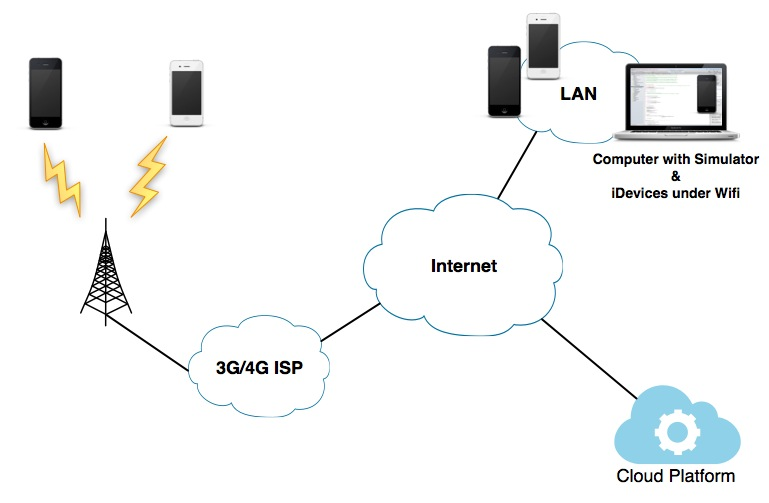
\includegraphics[width=0.8\textwidth]{./Images/test_env}
% \caption{Test Environment}
% \label{fig:test_env}
% \end{figure}

% Aliquam aliquet, est a ullamcorper condimentum, tellus nulla fringilla elit, a iaculis nulla turpis sed wisi. Fusce volutpat. Etiam sodales ante id nunc. Proin ornare dignissim lacus. Nunc porttitor nunc a sem. Sed sollicitudin velit eu magna. Aliquam erat volutpat. Vivamus egestas. Nunc tempor diam vehicula mauris. Nullam sapien eros, facilisis vel, eleifend non, auctor dapibus, pede \Cref{tab:network_profiles} used in the tests. The Network Link Conditioner allows to force/simulate fluctuations in fixed network segments.

% \begin{table}[htb]
% \centering
% \normalsize
%     \caption{Network Link Conditioner Profiles}
%     \label{tab:network_profiles}
% {\footnotesize
%     \begin{tabular}{ | c | c | c | c | }
%     \hline 
%     \textbf{Network Profile}	& \textbf{Bandwidth} & \textbf{Packets Droped} & \textbf{Delay}\\ \hline \hline
%     Wifi  & 40 mbps  &  0\%  &   1 ms \\ \hline
%     3G  & 780 kbps  &  0\%  &   100 ms \\ \hline 
%     Edge  & 240 kbps  &  0\%  &   400 ms \\ \hline
%     \end{tabular}
%     }
% \end{table}

% Aliquam aliquet, est a ullamcorper condimentum, tellus nulla fringilla elit, a iaculis nulla turpis sed wisi. Fusce volutpat. Etiam sodales ante id nunc. Proin ornare dignissim lacus. Nunc porttitor nunc a sem. Sed sollicitudin velit eu magna. Aliquam erat volutpat. Vivamus ornare est non wisi. Proin vel quam. Vivamus egestas. Nunc tempor diam vehicula mauris. Nullam sapien eros, facilisis vel, eleifend non, auctor dapibus, pede.
% % #############################################################################
% \section{Proin ornare dignissim lacus}
% Pellentesque habitant morbi tristique senectus et netus et malesuada fames ac turpis egestas. Vestibulum tortor quam, feugiat vitae, ultricies eget, tempor sit amet, ante. Donec eu libero sit amet quam egestas semper. Aenean ultricies mi vitae est. Mauris placerat eleifend leo. Quisque sit amet est et sapien ullamcorper pharetra. Vestibulum erat wisi, condimentum sed, commodo vitae, ornare sit amet, wisi. Aenean fermentum, elit eget tincidunt condimentum, eros ipsum rutrum orci, sagittis tempus lacus enim ac dui. Donec non enim in turpis pulvinar facilisis. Ut felis.

% Et ``optimistic'' nulla dui purus, eleifend vel, consequat non, dictum porta, nulla. Duis ante mi, laoreet ut, commodo eleifend, cursus nec, lorem. Aenean eu est. Etiam imperdiet turpis. Praesent nec augue. Curabitur ligula quam, rutrum id, tempor sed, consequat ac, dui $G_j$, nec ligula et lorem consequat ullamcorper $p$ ut mauris eu mi mollis luctus $j$, porttitor ut, \Cref{unchoke_gain}, uctus posuere justo:

% \begin{description}
%   \item[$N_j$] Is the number of times peer $j$ has been optimistically unchoked.
%   \item[$n_j$] Among the $N_j$ unchokes, the number of times that peer $j$ responded with unchoke or supplied segments to peer $p$.
%   \item[$C_{r[j]}$] The cooperation ratio of peer $j$. If peer $j$ never supplied peer $p$, the information of $C_{r[j]}$ may not be available.
%   \item[$C_{r (max)}$] The maximum cooperation ratio of peer $p$’s neighbors, i.e., $C_{r (max)} = max(C_r)$.
% \end{description}

% \begin{equation}
% \label{unchoke_gain}
%  G_j =
%   \begin{dcases}
%     \frac{n_j C_{r[j]}}{N_j} &\quad \text{if } n_j > 0\\
%     \frac{C_{r (max)}}{N_j + 1} &\quad \text{if } n_j = 0
%   \end{dcases}
% \end{equation}

% Cursus $C_{r (max)}$ conubia nostra, per inceptos hymenaeos $j$ gadipiscing mollis massa $N_j = 0$, unc ut dui eget nulla venenatis aliquet $G_j = C_{r (max)}$.

% Vestibulum accumsan eros nec magna. Vestibulum vitae dui. Vestibulum nec ligula et lorem consequat ullamcorper. Class aptent taciti sociosqu ad litora torquent per conubia nostra, per inceptos hymenaeos. Phasellus eget nisl ut elit porta ullamcorper. Maecenas tincidunt velit quis orci. Sed in dui. Nullam ut mauris eu mi mollis luctus. Class aptent taciti sociosqu ad litora torquent per conubia nostra, per inceptos hymenaeos. Sed cursus cursus velit. Sed a massa. 

% Both \Cref{fig:tx_layer_4,fig:tx_layer_5} Phasellus eget nisl ut elit porta ``perfect'' tincidunt. Class aptent taciti sociosqu ad litora torquent per conubia nostra.

% \begin{figure}[h]
% %\centering
%        \subfigure[Adaptation System Test 4]{\label{fig:tx_layer_4}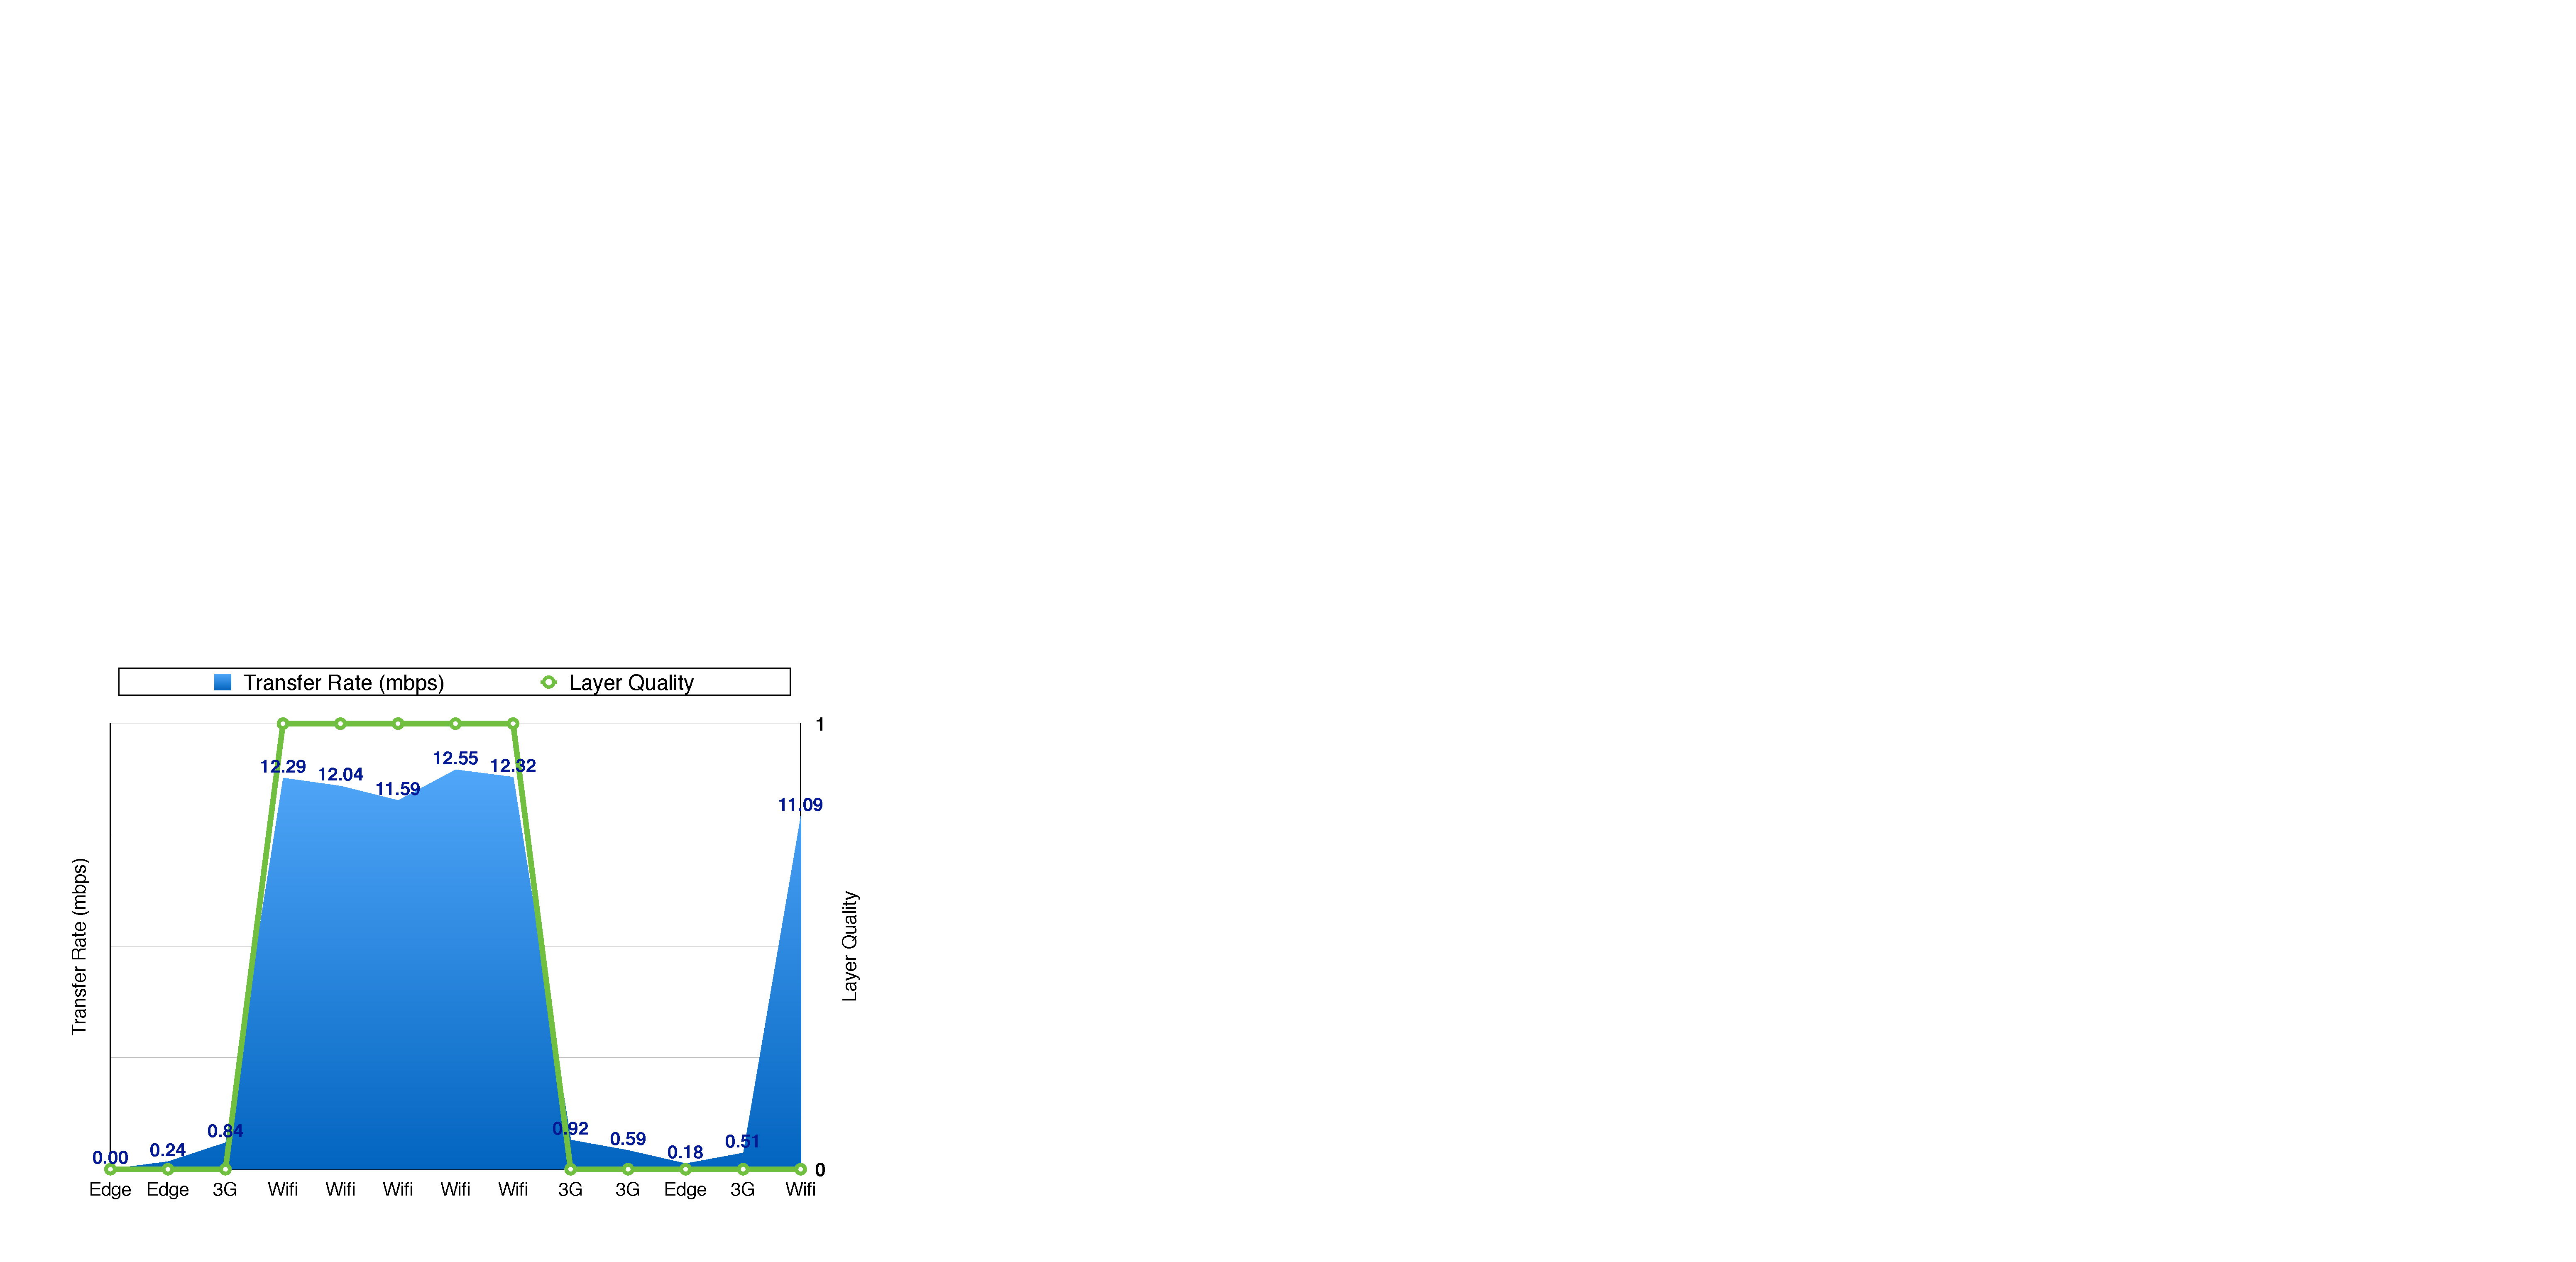
\includegraphics[width=0.5\textwidth]{./Images/tx_layer_4}}  
%    %    \centering 
%        \subfigure[Adaptation System Test 5]{\label{fig:tx_layer_5}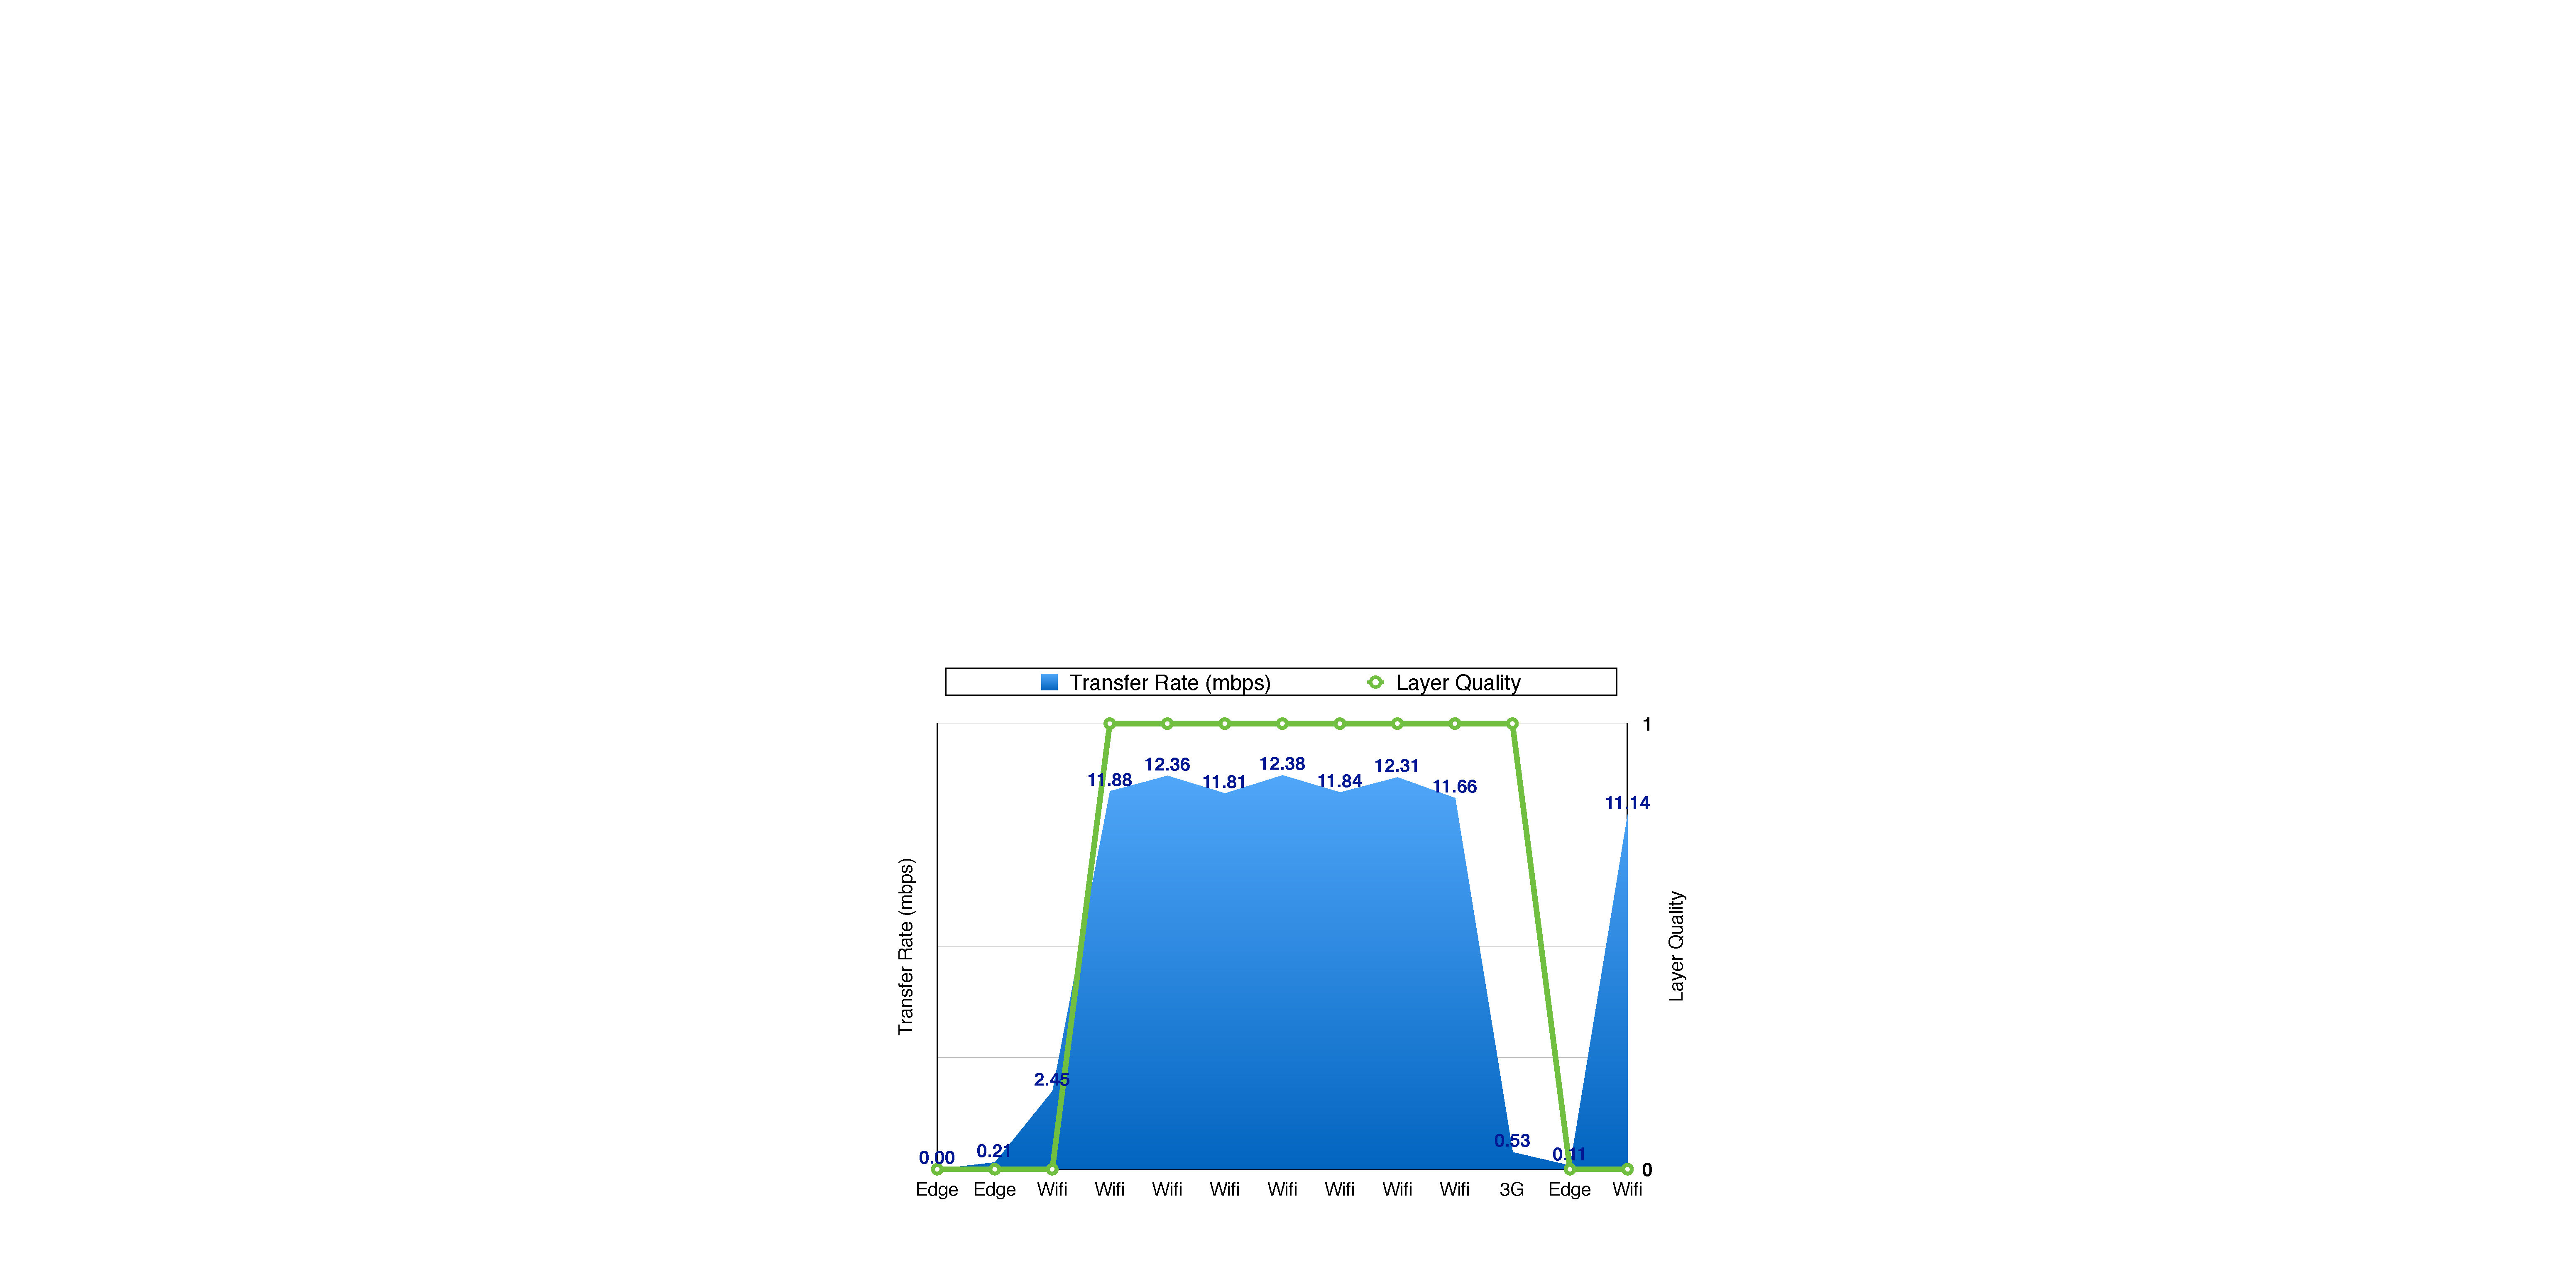
\includegraphics[width=0.5\textwidth]{./Images/tx_layer_5}}   
%         \caption{Adaptation System Behavior Test}
%         \label{fig:fig:adapt_behave_2}
% \end{figure}

% Cras sed ante. Phasellus in massa. Curabitur dolor eros, gravida et, hendrerit ac, cursus non, massa. Aliquam lorem. In hac habitasse platea dictumst. Cras eu mauris. Quisque lacus. Donec ipsum. Nullam vitae sem at nunc pharetra ultricies. Vivamus elit eros, ullamcorper a, adipiscing sit amet, porttitor ut, nibh. Maecenas adipiscing mollis massa. Nunc ut dui eget nulla venenatis aliquet. Sed luctus posuere justo. Cras vehicula varius turpis. Vivamus eros metus, tristique sit amet, molestie dignissim, malesuada et, urna.